%\newsection{Kapitel1}

%Hier den Inhalt mit \input einfügen und die folgenden Zeilen entfernen


%%%%%%%%%%%%%%%%%%%%%%%%%%%%%%%%%%%%%%%%%%%%%%%%% Anfang - Kapazität	 %%%%%%%%%%%%%%%%%%%%%%%%%%%%%%%%%%%%%%%%%%%%%%

	\section{Kapazität und Kondensator}
\s{
In der Elektrotechnik gibt es drei grundlegende Komponenten, mit denen das elektrische Verhalten von Bauteilen beschrieben werden kann.
Neben dem zuvor behandelten ohmschen Widerstand, gibt es noch die Kapazität und die Induktivität.
In diesem Abschnitt geht es um die Eigenschaft der Kapazität, sowie dem dazugehörigen Bauteil, dem Kondensator.
Der darauffolgende Abschnitt behandelt die Induktivität sowie das zugehörige Bauteil, die Spule.
}
%%%%%%%%%%%%%%%%%%%%%%%%%%%%%%%%%%%%%%%%%%%%%%%%% Anfang - Lernziele Kapazität	 %%%%%%%%%%%%%%%%%%%%%%%%%%%%%%%%%%%%%%%%%%%%%%
\begin{frame}
	\ftx{Lernziele: Kapazität und Kondensator}
\begin{Lernziele}{Kapazität und Kondensator}
	Die Studierenden
	\begin{itemize}
	\item können zwischen Kapazität und Kondensator differenzieren.
	\item kennen die wichtigsten Parameter rund um den Kondensator und die Kapazität.
	\item können die Kapazität eines Kondensators berechnen.
\end{itemize}
\end{Lernziele}

\speech{03_Kapazitaet_und_Kondensator}{1}{
Im nun folgenden Abschnitt beschäftigen wir uns mit dem Begriff der Kapazität und dem damit verbundenen Bauteil – dem Kondensator. 
Am Ende dieses Abschnittes sollten Sie zwischen Kapazität und Kondensator differenzieren können. 
Sie kennen die wichtigsten Parameter rund um den Kondensator und die Kapazität und 
Sie können die Kapazität eines einfachen Plattenkondensators berechnen.    
}

\end{frame}

%%%%%%%%%%%%%%%%%%%%%%%%%%%%%%%%%%%%%%%%%%%%%%%%% Ende - Lernziele Kapazität	 %%%%%%%%%%%%%%%%%%%%%%%%%%%%%%%%%%%%%%%%%%%%%%

	\subsection{Die elektrische Kapazität $C$}
\s{
	Die elektrische Kapazität ist die Fähigkeit eines Objektes, elektrische Energie in Form eines elektrischen Feldes, zu speichern.
	Diese Eigenschaft kommt zustande, sobald elektrische Ladungsträger ungleich verteilt sind und sich zwischen den Bereichen
	ein elektrisches Feld ausbildet. Das Formelzeichen der Kapazität ist $C$ (capacity) während die Einheit in Farad ($F$) angegeben wird.

}% nur im Skript

\s{
Das einfachste und geläufigste Beispiel, an dem die Kapazität erklärt werden kann, ist der Plattenkondensator.
Bei dieser Art des Kondensators liegen sich zwei leitfähige Platten gegenüber, welche jeweils mit einem anderen Potential beaufschlagt werden.
In Abbildung \ref{fig:idealer Kondensator} ist ein Kondensator mit idealisiertem Feldverlauf dargestellt.
}
%%%%%%%%%%%%%%%%%%%%%%%%%%%%%%%%%%%%%%%%%%%%%%%%% Anfang - Grafik idealer Kondensator	 %%%%%%%%%%%%%%%%%%%%%%%%%%%%%%%%%%%%%%%%%%%%%%
\begin{frame}
	\ftx{Die elektrische Kapazität}
	\b{
		\begin{itemize}
			\item Der ideale Plattenkondensator
			\end{itemize}
	}
	\begin{figure}[H]
		\centering
			\includesvg[width=0.6\textwidth]{Idealer_Plattenkondensator}
			\s{\caption{\textbf{Idealer Plattenkondensator mit idealisierten Feldverlauf.} Der Kondensator
			speichert elektrische Energie in einem elektrischen Feld was idealisiert zwischen den Platten dargestellt ist und hat eine konstante Kapazität \( C \), die nur von der Fläche der Platten und dem Abstand zwischen ihnen abhängt.}}
			\label{fig:idealer Kondensator}
		\end{figure}
%%%%%%%%%%%%%%%%%%%%%%%%%%%%%%%%%%%%%%%%%%%%%%%%% Ende - Grafik idealer Kondensator	 %%%%%%%%%%%%%%%%%%%%%%%%%%%%%%%%%%%%%%%%%%%%%%
\s{
Aufgrund der unterschiedlichen Potentiale auf den Platten, bildet sich von der höheren zur geringer geladenen Platte ein elektrisches Feld aus.
Im idealen Fall wird angenommen, dass sich außerhalb der Kondensatorplatten kein Feld ausbildet.
In der Realität sammeln sich an den seitlichen Rändern der Platten ebenfalls Ladungsträger, welche zu komplizierteren Feldverteilungen führen.
In Abbildung \ref{fig:realer Kondensator} ist die Grafik eines solchen realen Plattenkondensators dargestellt.
}% nur im Skript

\speech{03_Kapazitaet_und_Kondensator}{2}{
Die einfachste Form eines Kondensators ist der sogenannte Plattenkondensator. 
Bei dem hier dargestellten idealen Plattenkondensator stehen sich zwei leitfähige Platten parallel gegenüber. 
Zwischen diesen leitfähigen Platten ist ein Isolator – ein sogenanntes Dielektrikum. 
Das heißt, es kann kein Strom zwischen diesen beiden Platten fließen. 
Wenn es uns nun z. B. durch das Anlegen einer Spannung an die beiden Platten gelingt, eine Ladungsträgertrennung zu erzeugen – 
hier dargestellt durch positive Ladungen auf der linken Seite und negative Ladungen auf der rechten Seite – 
dann baut sich ein elektrisches Feld E auf, das in der Darstellung in rot eingezeichnet ist.    
}

\end{frame}
%%%%%%%%%%%%%%%%%%%%%%%%%%%%%%%%%%%%%%%%%%%%%%%%% Anfang - Grafik realer Kondensator	 %%%%%%%%%%%%%%%%%%%%%%%%%%%%%%%%%%%%%%%%%%%%%%
\begin{frame}
	\ftx{Die elektrische Kapazität}
	\b{
		\begin{itemize}
			\item Der reale Plattenkondensator
			\end{itemize}
	}
	\begin{figure}[H]
		\centering
			\includesvg[width=0.6\textwidth]{Realer_Plattenkondensator}
			\s{\caption{\textbf{Realer Kondensator mit realem Feldverlauf.} Im Gegensatz zum idealen Kondensator treten
			  Randfelder und Verluste auf, die die tatsächliche Kapazität und das elektrische Verhalten beeinflussen.}}

			\label{fig:realer Kondensator}
		\end{figure}

\speech{03_Kapazitaet_und_Kondensator}{3}{
In der Realität ist das elektrische Feld jedoch nicht nur exakt zwischen den Platten vorhanden und senkrecht. 
Es gibt darüber hinaus sogenannte Streufelder, die an den Rändern der Platten auftreten. 
Da die Platten aus leitfähigem Material bestehen, müssen sämtliche Feldlinien, die austreten bzw. eintreten, senkrecht auf den entsprechenden Oberflächen stehen. 
Deshalb entstehen gebogene Feldlinienverläufe am Rand. 
Auch die oben und unten angedeuteten Feldlinien sind geschlossen – 
sie sind hier zur besseren Lesbarkeit nicht vollständig dargestellt, weil das sonst die Übersichtlichkeit zerstören würde.    
}

\end{frame}
%%%%%%%%%%%%%%%%%%%%%%%%%%%%%%%%%%%%%%%%%%%%%%%%% Ende - Grafik realer Kondensator	 %%%%%%%%%%%%%%%%%%%%%%%%%%%%%%%%%%%%%%%%%%%%%%
\begin{frame}[t]
	\ftx{Die elektrische Kapazität}
\b{
	\begin{minipage}[t]{1\textwidth}
	\begin{equation*}
		[C] =  1\, \text{Farad} = 1\, \text{F} =  1\,\, \frac{\text{C}}{\text{V}} = 1\, \frac{\text{A} \text{s}}{\text{V}} \label{eq:cqu}
	\end{equation*}
	\vspace{0.1cm}
	\begin{equation*}
		C = \frac{Q}{U}
	\end{equation*}
	\end{minipage}
%%% aus Einführung in zeitabhängige Vorgänge (MH)
	\vspace{2cm}
	\only<2->{\begin{equation*}
		Q = C \cdot U \quad \Rightarrow \quad C = \frac{Q}{U} = \frac{\varepsilon \cdot \iint \vec{E} \cdot \mathrm{d}\vec{A}}{\int \vec{E}\mathrm{d}\vec{s}}
	\end{equation*}}
}
 % ToDo: Hillgärtner: 	Die Folie enthält die Formel C = Q / U sowohl oben als auch unten, was redundant wirkt. 
% 						Eventuell sollte die Darstellung überarbeitet werden. 
% 						Außerdem ist fraglich, ob wir die Feldstärke E wirklich auf dieser Folie mit aufführen müssen – 
% 						das ist womöglich an dieser Stelle verwirrend oder nicht nötig. 

\speech{03_Kapazitaet_und_Kondensator}{4}{ %ToDo: only 1
Ein solcher Plattenkondensator baut ein elektrisches Feld auf. 
In diesem Feld kann elektrische Energie gespeichert werden. 
Das Maß für die Fähigkeit, elektrische Energie im Feld eines Kondensators zu speichern, ist die Kapazität. 
Die Kapazität wird mit dem Buchstaben C abgekürzt. 
Die Einheit der Kapazität ist das Farad (F). 
1 Farad bedeutet, dass 1 Coulomb an Ladung gespeichert wird, wenn 1 Volt Spannung anliegt. 
Formelmäßig also: C = Q / U. 
Alternativ in SI-Einheiten: Farad = As / V (Ampere-Sekunde pro Volt).    
}

\speech{03_Kapazitaet_und_Kondensator}{5}{ %ToDo: only 2
Wir können die Formel C = Q / U auch umstellen zu Q = C × U.     
}


\end{frame}
\s{
	In vielen Fällen kann das reale Verhalten jedoch vernachlässigt werden, was die Berechnungen deutlich vereinfacht.
	Aus dem Grund wird im Folgenden nurnoch von idealisierten Kondensatoren ausgegangen.


	Die Kapazität ist definiert als das Verhältnis der gespeicherten elektrischen Ladung $Q$ zur angelegten Spannung $U$.
	Je höher die Kapazität eines Kondensators ist, desto mehr Ladung kann er bei einer gegebenen Spannung speichern.

%%%%%%%%%%%%%%%%%%%%%%%%%%%%%%%%%%%%%%%%%%%%%%%%% Anfang - Formeln Kapazität	 %%%%%%%%%%%%%%%%%%%%%%%%%%%%%%%%%%%%%%%%%%%%%%
	\begin{equation*}
		[C] =  1\, \text{Farad} = 1\, \text{F} =  1\,\, \frac{\text{C}}{\text{V}} = 1\, \frac{\text{A} \text{s}}{\text{V}} \label{eq:cqu}
	\end{equation*}
	\vspace{0.1cm}
	\begin{equation}
		C = \frac{Q}{U}
	\end{equation}
%%% aus Einführung in zeitabhängige Vorgänge (MH)
	\begin{equation}
		Q = C \cdot U \quad \Rightarrow \quad C = \frac{Q}{U} = \frac{\varepsilon \cdot \iint \vec{E} \cdot \mathrm{d}\vec{A}}{\int \vec{E}\mathrm{d}\vec{s}} \label{eq:qcu2}
	\end{equation}
}

%%%%%%%%%%%%%%%%%%%%%%%%%%%%%%%%%%%%%%%%%%%%%%%%% Ende - Formeln Kapazität	 %%%%%%%%%%%%%%%%%%%%%%%%%%%%%%%%%%%%%%%%%%%%%%
	\subsection{Der Kondensator als Bauelement}

\s{
	Die Eigenschaften der Kapazität werden in verschiedenen Bereichen der Elektrotechnik bewusst genutzt.
	Die Nutzbarmachung dieser Eigenschaften erfolgt mit Hilfe von Kondensatoren. Es gibt sie in verschiedenen Ausführungen.
	Abbildung \ref{fig:Verschiedene Kondensatoren} zeigt einige Beispiele von THT- bis hin zu SMD-Bauteilen.
}

%%%%%%%%%%%%%%%%%%%%%%%%%%%%%%%%%%%%%%%%%%%%%%%%% Anfang - Bild versch. Kondensatoren	%%%%%%%%%%%%%%%%%%%%%%%%%%%%%%%%%%%%%%%%%%%%%%

%%% Quelle einfügen!

\begin{frame}
	\ftx{Der Kondensator als Bauelement}
	\b{
		\begin{itemize}
			\item Verschiedene Arten und Bauformen von Kondensatoren
		\end{itemize}
	}
	\begin{figure}[H]
		\centering
		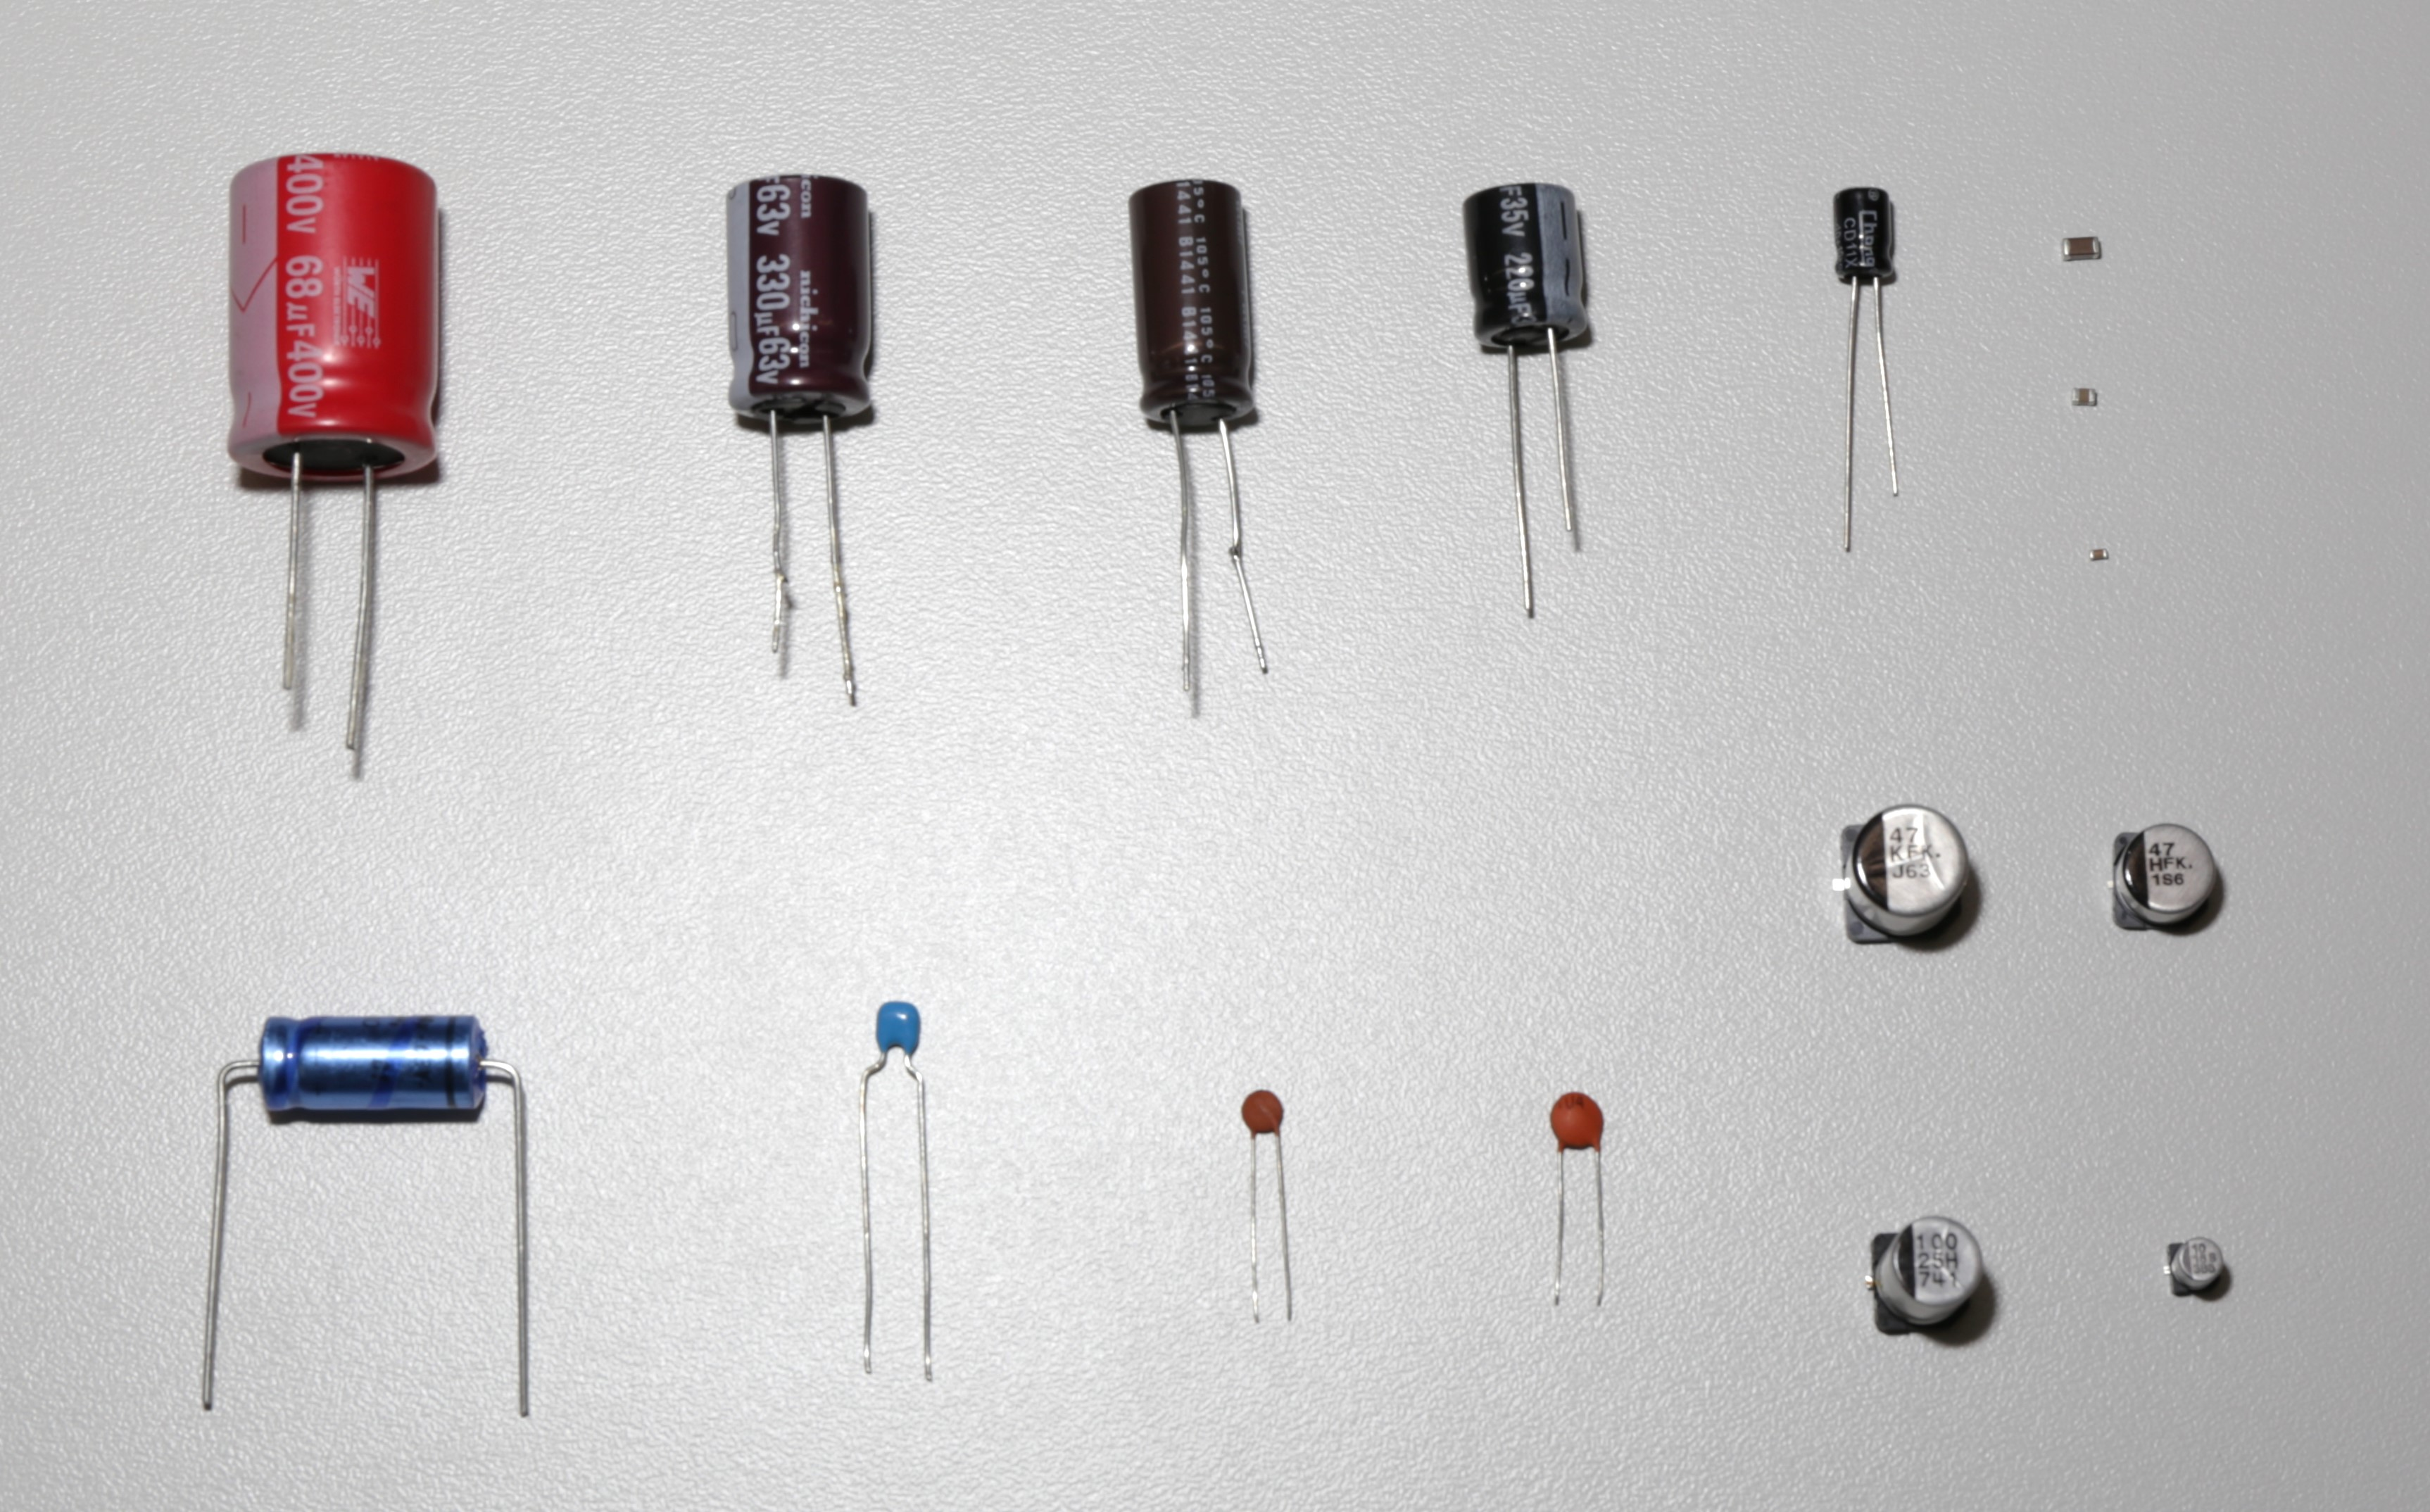
\includegraphics[width=0.7\textwidth]{ko}
		\s{\caption{\textbf{Verschiedene Arten und Bauformen von Kondensatoren.} Darunter Keramik- und Elektrolytkondensatoren.
		 Diese variieren in Größe, Kapazität und Spannung, um unterschiedlichen Anwendungen gerecht zu werden.}}

		\label{fig:Verschiedene Kondensatoren}
	\end{figure}

\speech{03_Kapazitaet_und_Kondensator}{6}{
Auf dem hier dargestellten Foto sehen Sie verschiedene Ausführungen von Bauteilen. Bis auf den ganz rechten Rand sind das alles Durchsteckelemente, also P2-Bauteile, was gerade bei Kondensatoren relativ häufig vorkommt, da diese räumlich groß sein müssen, um hinreichende Kapazitäten zu haben. Wir werden später sehen, dass je größer die Fläche ist, die wir haben, und je kleiner der Abstand, desto größer wird die Kapazität, weil letztlich das elektrische Bild natürlich größer wird und die Ladungsmenge, die gespeichert werden kann, größer wird. 
Weswegen Sie auch hier sehr schön sehen, dass wir gewisse Zusammenhänge haben. Der rote Kondensator oben links ist ein 400 Volt, 68 µF Kondensator. Der ist räumlich sehr viel größer als der 63 Volt, 330 µF Kondensator rechts daneben, der schwarze. Der schwarze Kondensator hat eine Kapazität, die rund 4,5 bis 5 Mal größer ist als die des roten Kondensators und ist räumlich trotzdem kleiner. Wie kann das erreicht werden? Indem der Abstand zwischen den Platten deutlich kleiner ist, weswegen er auch nur eine kleine Spannung aushalten kann. 
Denn die Platten müssen ja voneinander isoliert sein. Das heißt, man wickelt dort ein Material ein, zwischen die Platten ein in Elektrolyt getränktes Material. Das sind sogenannte Elektrolytkondensatoren. Das hat nur eine gewisse Dicke und hinzufolge auch nur eine gewisse Spannungsfestigkeit. 
Das heißt, wenn Sie Kondensatoren haben möchten, die hohe Spannung aushalten und gleichzeitig aber hohe Kapazitätswerte haben, dann werden das räumlich extrem große Bauteile. Unten ist eine andere Technologie. Das sind Keramik- und Tantalkondensatoren, die meistens deutlich kleinere Kapazitätswerte haben, dafür aber elektrisch häufig sehr viel bessere Eigenschaften haben, sodass die abhängig von der Anwendung gewählt werden. Ganz oben rechts die kleinen Chips. Das sind klassische SMD-Bauteile. Wieder ohne Beinchen, das heißt deutlich weniger parasitäre Effekte, aber auch kleinere Kapazitätswerte. Und unten rechts sehen Sie Elektrolytkondensatoren als SMD-Kondensatoren, die eben auch direkt auf der Platine montiert werden.
    
}

	\end{frame}
	%%%%%%%%%%%%%%%%%%%%%%%%%%%%%%%%%%%%%%%%%%%%%%%%% Ende - Bild versch. Kondensatoren	 %%%%%%%%%%%%%%%%%%%%%%%%%%%%%%%%%%%%%%%%%%%%%%
\s{
	Darüber hinaus gibt es sie aber auch in deutlich kleineren bzw. deutlich größeren Dimensionen.
	In der Hochfrequenztechnik werden Kapazitäten beispielsweise lediglich durch das Design der Leiterplatten realisiert,
	während Kondensatoren für industrielle oder enegietechnische Anwendungen mehrere Zentimeter bis Meter groß werden können.

	Was alle Kondensatoren verbindet, ist ihre Fähigkeit, die Eigenschaft der Kapazität nutzbar zu machen,
	wie es im folgenden Schaltbild \ref{fig:idealer Kondensator_ESB} dargestellt ist.
	Dieses Schaltbild repräsentiert jedoch nur die idealisierte, nutzbare Kapazität.
}
%%%%%%%%%%%%%%%%%%%%%%%%%%%%%%%%%%%%%%%%%%%%%%%%% Anfang - Schaltzeichen Kapazität U,I	%%%%%%%%%%%%%%%%%%%%%%%%%%%%%%%%%%%%%%%%%%%%%%
\begin{frame}[t]
	\ftx{Der Kondensator als Bauelement}
	% idealer Kondensator
\b{
	\begin{itemize}
	\item Idealer Kondensator
\end{itemize}
\begin{figure}[h]
	\begin{center}
	\begin{circuitikz}
    \draw (-1,0) to[short,o-] (0,0);
    \draw (0,0)   to [C,i,v, name=C, l={$C$}] (0,-2)
    to [short,-o] (-1,-2);
    \iarrmore{C}{$i_\mathrm{C}(t)$};
    \varrmore{C}{$u_\mathrm{C}(t)$};

\end{circuitikz}

	\label{fig:idealer Kondensator_ESB}
	\end{center}
	\end{figure}

	\only<2->{

\begin{itemize}
	\item Ersatzschaltbild eines realen Kondensators
\end{itemize}
\begin{figure}[H]
	\begin{center}
	\begin{circuitikz}[european resistors]
    \draw (0,0)   to [C,i,v, name=C,o-, l={$C$}] (2.4,0)
    (2,0)   to [R,v, name=R, l={$R_\mathrm{s}$}] (4,0)
    (4,0)   to [L,v, name=L, l={$L_\mathrm{s}$}] (6,0)
    (6,0)   to [short,-o] (6.25,0);
    \iarrmore{C}{$i_\mathrm{C}(t)$};
    \varrmore{C}{$u_\mathrm{C}(t)$};
    \varrmore{R}{$u_\mathrm{R}(t)$};
    \varrmore{L}{$u_\mathrm{L}(t)$};

\end{circuitikz}
	\label{fig:realer Kondensator_ESB}
	\end{center}
	\end{figure}
}
}

\speech{03_Kapazitaet_und_Kondensator}{7}{ % ToDo: only 1
In einer idealen Welt hat ein Kondensator tatsächlich nur die gewünschte Kapazität. An dieser gewünschten Kapazität liegt eine Spannung an, die jetzt hier als zeitlich variable Spannung anliegt. Und dann fließt auch tatsächlich ein zeitlich variabler Strom durch eben genau diese Kapazität. Ein Strom IC von T. 
}

\speech{03_Kapazitaet_und_Kondensator}{8}{ % ToDo: only 2
Leider Gottes schlagen aber die parasitären Elemente bei einem realen Kondensator sehr stark ins Gewicht. Das einfachste Ersatzschadbild eines realen Kondensators ist die gewünschte Kapazität in Reihe zu einem Serienwiderstand und einer Serieninduktivität. Der Serienwiderstand, den können wir uns relativ leicht erklären, denn irgendwo haben wir ja gerade schon auf dem Bild gesehen, dass wir immer Anschlussleitungen haben. Diese Anschlussleitungen haben immer einen ohmschen Widerstand. Dieser ohmsche Widerstand, R, verändert natürlich das Verhalten des Kondensators. Das wäre meistens noch sehr gut zu verschmerzen. 
Viel problematischer ist aber die in Serie liegende Induktivität. Im späteren Verlauf, in anderen Modulen, werden Sie das Frequenzverhalten von Kapazität und Induktivität mehr kennenlernen. Vereinfacht besprochen leitet ein Kondensator den Strom immer besser, je höher die Frequenz ist. Wohingegen die Induktivität den Strom immer schlechter leitet mit höher werdender Frequenz. 
Sodass wir hier im Prinzip gegensätzliche Bauteileigenschaften haben. In der Realität ist es tatsächlich so, dass ein Kondensator abhängig von seinem Aufbau irgendwann nicht mehr die gewünschte Kapazität schaltungstechnisch darstellt, sondern sich eher wie eine Induktivität verhält. Da die parasitäre Induktivität, die ihr da alles stellt, als LS dominant wird. Und je größer das Bauelement geometrisch, desto schlechter ist dieses Verhältnis zueinander. 
D.h. die gerade dargestellten Elektrolytkondensatoren, die räumlich sehr groß sind, die können Sie tatsächlich nur bei relativ niedrigen Frequenzen verwenden. Da ist dann der kapazitive Anteil noch dominant. D.h. diese Kondensatoren werden z.B. benutzt, um Eingangsspannung zu stabilisieren. Wohingegen für hochfrequentere Anwendungen, Filterschaltung und so, kommen eher die ganz kleinen SMD-Bauteile zum Tragen, weil dann das kapazitive Verhalten des Kondensators bis hin zu höheren Frequenzen garantiert werden kann.
}

\end{frame}
\s{
	\begin{figure}[h]
		\begin{center}
		\begin{circuitikz}
    \draw (-1,0) to[short,o-] (0,0);
    \draw (0,0)   to [C,i,v, name=C, l={$C$}] (0,-2)
    to [short,-o] (-1,-2);
    \iarrmore{C}{$i_\mathrm{C}(t)$};
    \varrmore{C}{$u_\mathrm{C}(t)$};

\end{circuitikz}
		\caption{\textbf{Schaltelement eines idealen Kondensators.} Zeigt den Spannungsabfall über dem Kondensator und den Stromfluss durch ihn.}

		\label{fig:idealer Kondensator_ESB}
		\end{center}
		\end{figure}

%%%%%%%%%%%%%%%%%%%%%%%%%%%%%%%%%%%%%%%%%%%%%%%%% Ende - Schaltzeichen Kapazität U,I	 %%%%%%%%%%%%%%%%%%%%%%%%%%%%%%%%%%%%%%%%%%%%%%

	Für eine realitätsgetreue Nachbildung der Schaltung ist es wichtig den Kondensator als Bauteil vollständig zu beschreiben.
	Dies wird mit Hilfe eines Ersatzschaltbildes gemacht, welches auch die ungewollten, also parasitären Eigenschaften
	des Bauteils, nachbildet. Abbildung \ref{fig:realer Kondensator_ESB} zeigt ein solches Ersatzschaltbild.

%%%%%%%%%%%%%%%%%%%%%%%%%%%%%%%%%%%%%%%%%%%%%%%%% Anfang - ESB Kondensator	 %%%%%%%%%%%%%%%%%%%%%%%%%%%%%%%%%%%%%%%%%%%%%%
% realer Kondensator


		\begin{figure}[H]
			\begin{center}
			\begin{circuitikz}[european resistors]
    \draw (0,0)   to [C,i,v, name=C,o-, l={$C$}] (2.4,0)
    (2,0)   to [R,v, name=R, l={$R_\mathrm{s}$}] (4,0)
    (4,0)   to [L,v, name=L, l={$L_\mathrm{s}$}] (6,0)
    (6,0)   to [short,-o] (6.25,0);
    \iarrmore{C}{$i_\mathrm{C}(t)$};
    \varrmore{C}{$u_\mathrm{C}(t)$};
    \varrmore{R}{$u_\mathrm{R}(t)$};
    \varrmore{L}{$u_\mathrm{L}(t)$};

\end{circuitikz}
			\caption{\textbf{Ersatzschaltbild eines realen Kondensators.} Der ideale Kondensator $C$ wird durch eine Serien-Induktivität
			 $L_\mathrm{s}$ und einen Serien-Widerstand $R_\mathrm{s}$ ergänzt, um parasitäre Effekte zu berücksichtigen.}

			\label{fig:realer Kondensator_ESB}
			\end{center}
			\end{figure}
}

%%%%%%%%%%%%%%%%%%%%%%%%%%%%%%%%%%%%%%%%%%%%%%%%% Ende - ESB Kondensator	 %%%%%%%%%%%%%%%%%%%%%%%%%%%%%%%%%%%%%%%%%%%%%%
\s{
	Im Ersatzschaltbild des Kondensators werden nicht nur die nutzbare Kapazität, sondern auch die parasitären Eigenschaften
	berücksichtigt, die in realen Kondensatoren auftreten. Diese parasitären Eigenschaften entstehen beispielsweise durch die
	Induktivität der Anschlüsse und die ohmschen Verluste im Material.
	Das modellierte Ersatzschaltbild ermöglicht es, diese Effekte im Schaltungsentwurf zu berücksichtigen
	und das Schaltverhalten besser vorherzusagen.
}
%%%%%%%%%%%%%%%%%%%%%%%%%%%%%%%%%%%%%%%%%%%%%%%%%%%% Anfang Merksatz - Kondensator %%%%%%%%%%%%%%%%%%%%%%%%%%%%%%%%%%%%%%%%%
\begin{frame}
	\ftx{Merksatz: Der Kondensator als Bauelement}
	\begin {Merksatz}{}
		 Der Kondensator ist der verzweifelte Versuch eine Kapazität nachzubilden.
	\end {Merksatz}

	\speech{03_Kapazitaet_und_Kondensator}{9}{
Wir können uns also merken, dass der Kondensator immer nur der verzweifelte Versuch ist, eine Kapazität nachzubilden. Wir hatten das ja schon beim Widerstand, dass das Bauteil Widerstand eben noch andere Eigenschaften hat, als nur die gewünschte Eigenschaft des ungewünschten Widerstandes. So ist das letztlich beim Kondensator auch. Und diese ungewünschten Eigenschaften fallen insbesondere dann ins Gewicht, wenn sie hingehen zu höheren Frequenzen.    
}

	\end{frame}
%%%%%%%%%%%%%%%%%%%%%%%%%%%%%%%%%%%%%%%%%%%%%%%%%%%% Ende Merksatz - Kondensator %%%%%%%%%%%%%%%%%%%%%%%%%%%%%%%%%%%%%%%%%
%%%%%%%%%%%%%%%%%%%%%%%%%%%%%%%%%%%%%%%%%%%%%%%%% Anfang - Dielektrikum	 %%%%%%%%%%%%%%%%%%%%%%%%%%%%%%%%%%%%%%%%%%%%%%
\subsection{Das Dielektrikum}
\s{
Das Dielektrium ist, wie der Name bereits impliziert, ein dielektrisches, also elektrisch nicht leitfähiges Material.
Da jedes Material aus Atomen besteht und alle Atomrümpfe mit Elektronen versehen sind (Elektronenhülle),
wirkt sich entsprechend auch ein elektrisch nicht leitfähiges Material auf das Verhalten des elektrischen Feldes aus.
Sobald ein solches Material zwischen die Platten eines Kondensators eingefügt wird, ändern sich demnach auch die Eigenschaften des Kondensators.
In Abbildung \ref{fig:idealer Kondensator mit Dielektrikum} ist anhand der unterbrochenen Pfeilung des elektrischen Feldes
das unterschiedliche Verhalten zu erkennen. Die elektrische Flussdichte D ist eine Hilfsgröße, welche materialunabhängig ist,
auf welche in Abschnitt 1.3.4 noch eingegangen wird.
}
%%%%%%%%%%%%%%%%%%%%%%%%%%%%%%%%%%%%%%%%%%%%%%%%% Anfang - Grafik Dielektrikum	 %%%%%%%%%%%%%%%%%%%%%%%%%%%%%%%%%%%%%%%%%%%%%%
\begin{frame}
	\ftx{Das Dielektrikum}
\begin{figure}[H]
	\centering
		\includesvg[width=0.6\textwidth]{Idealer_Plattenkondensator_Dielektrikum}
		\s{\caption{\textbf{Idealer Kondensator mit Dielektrikum.} Der Kondensator besteht aus zwei Platten, zwischen denen sich ein Dielektrikum befindet. Das Dielektrikum
		 ist ein nicht leitendes Material, das die elektrische Feldstärke reduziert und die Kapazität des Kondensators erhöht, indem es die Relative Dielektrizitätskonstante erhört.}}
		\label{fig:idealer Kondensator mit Dielektrikum}
	\end{figure}

\speech{03_Kapazitaet_und_Kondensator}{10}{
Ich hatte ja bereits gesagt, dass die beiden Platten voneinander isoliert werden müssen. Und dies kann im einfachsten Fall mit Luft als Dielektrikon passieren. Es kann aber auch ein dielektrischer Stoff eingeführt werden, das sogenannte Dielektrikon, hier in dunkelgrau dargestellt. Wir haben dann durchgehend gleich, sowohl im Dielektrikon als auch in der Luft, die elektrische Flussdichte d. Daraus ergibt sich als nicht-kontinuierlichen Teil die elektrische Feldstärke e, die im Dielektrikon deutlich größer werden wird als außerhalb. Was erreichen wir damit? Wir erreichen damit letztlich, dass die Kapazität unseres Kondensators sich erhöht, nämlich durch Volatilisationseffekte und ähnliches.    
}

\end{frame}
% Vielleicht an dieser Stelle Einschub zu Dielektrikum,
% Permeativität, was das ist, Zusammenhang zum Wellenwiderstand und zur Lichtgeschwindigkeit.

%%%%%%%%%%%%%%%%%%%%%%%%%%%%%%%%%%%%%%%%%%%%%%%%% Ende - Grafik Dielektrikum	 %%%%%%%%%%%%%%%%%%%%%%%%%%%%%%%%%%%%%%%%%%%%%%
\s{
Die Eigenschaften des Dielektrikums sind materialspezifisch und werden durch die Dielektrizitätszahl $\varepsilon_\mathrm{r}$ quantifiziert.
In Tabelle \ref{tab:dielektrizität} sind Beispiele einiger Dielektrika und deren $\varepsilon_\mathrm{r}$, aufgeführt:
}
%%%%%%%%%%%%%%%%%%%%%%%%%%%%%%%%%%%%%%%%%%%%%%%%% Anfang - Tabelle epsylon	 %%%%%%%%%%%%%%%%%%%%%%%%%%%%%%%%%%%%%%%%%%%%%%
\begin{frame}[t]
	\ftx{Das Dielektrikum}
	\b{
		\begin{itemize}
			\item Relative Dielektrizitätszahl verschiedener Materialien
		\end{itemize}
		\vspace{1cm}
	}
%%%%% Dielektrizitätszahl Einfache Tabelle
\begin{table}[H]
\centering
\resizebox{0.3\textwidth}{!}{%
\begin{tabular}{lc}
\toprule
\textbf{Material} & \textbf{\boldmath$\varepsilon_\mathrm{r}$} \\
\midrule
Vakuum & 1 \\
Luft (bei STP) & 1.0006 \\
Kunststoff (PE) & 2.25-2.3 \\
Glas & 3-10 \\
Keramik & 5-300 \\
Silizium & 11.7 \\
Tantaloxid & 25-30 \\
Wasser & 81 \\
\bottomrule
\end{tabular}%
}
\s{\caption{\textbf{Relative Dielektrizitätszahl verschiedener Materialien.} Diese dimensionslose Zahl gibt an,
wie stark das elektrische Feld in einem Material im Vergleich zum Vakuum beeinflusst wird. Sie ist ein Maß für die Fähigkeit des Materials, elektrische Ladung zu speichern.
Materialien mit einer höheren Dielektrizitätszahl erhöhen die Kapazität eines Kondensators, da sie die elektrische Feldstärke im Inneren verringern.}}
\label{tab:dielektrizität}
\end{table}

\speech{03_Kapazitaet_und_Kondensator}{11}{
Wir geben diese Möglichkeit der Erhöhung des elektrischen Feldes in einer elektrischen Flussdichte an über die Dielektrizitätszahlen. Wir müssen irgendwann die Dielektrizität, die Permeabilität, streiche das. Die relative Dielektrizitätszahl geht quasi an, wie viel das elektrische Feld erstärkt wird. Vakuum hat eine Dielektrizitätszahl von 1, Luft ziemlich genau von 1, wobei der häufig verwendete Kunststoff PE irgendwo so bei 2,3 liegt. Aber wir können auch Keramiken finden, die bis zu 300 als Dielektrizitätszahl haben oder Tantaloxid von 25 bis 30. Wasser ist ebenfalls ein sehr gutes Dielektrikum. Das Problem bei Wasser ist nur, dass es bei kleinsten Verunreinigungen bereits elektrisch leitfähig werden wird und damit diese die elektrischen Eigenschaften verliert.    
}

\end{frame}

%%%%% Kästchen Tabelle

% \begin{table}[H]
%     \centering
%     \begin{tabular}{|l|c|}
%         \hline
%         \textbf{Material} & \textbf{\boldmath$\varepsilon_\mathrm{r}$} \\
%         \hline
%         Vakuum & 1 \\
%         \hline
%         Luft (bei STP) & 1.0006 \\
%         \hline
%         Kunststoff (PE) & 2.25-2.3 \\
%         \hline
%         Glas & 3-10 \\
%         \hline
%         Keramik & 5-300 \\
%         \hline
%         Silizium & 11.7 \\
%         \hline
%         Tantaloxid & 25-30 \\
%         \hline
%         Wasser & 81 \\
%         \hline
%     \end{tabular}
%     \caption{Dielektrizitätszahl verschiedener Materialien}
%     \label{tab:dielektrizität}
% \end{table}
%%%%%%%%%%%%%%%%%%%%%%%%%%%%%%%%%%%%%%%%%%%%%%%%% Ende - Tabelle epsylon	 %%%%%%%%%%%%%%%%%%%%%%%%%%%%%%%%%%%%%%%%%%%%%%
\s{
	Zur vollständigen Beschreibung der Materialeigenschaften des Dielektrikums wird neben der Dielektrizitätszahl noch die elektrische Feldkonstante $\varepsilon_\mathrm{0}$ benötigt.
	Dabei handelt es sich um das dielektrische Verhalten des elektrischen Feldes im Vakuum. Während die Dielektrizitätszahl $\varepsilon_\mathrm{r}$ einheitslos ist,
	bringt die elektrische Feldkonstante die Einheit $\frac{\text{As}}{\text{Vm}}$ mit. Sie wird mit der relativen Dielektrizitätszahl multipliziert was zusammen
	die Dielektrizitätskonstante $\varepsilon$ ergibt.
}
%%%%%%%%%%%%%%%%%%%%%%%%%%%%%%%%%%%%%%%%%%%%%%%%%%%% Anfang Formel epsylon und Legende %%%%%%%%%%%%%%%%%%%%%%%%%%%%%%%%%
\begin{frame}
	\ftx{Das Dielektrikum}
	\b{
		\begin{equation*}
			[\boldsymbol\varepsilon] = 1\,\frac{\text{Farad}}{\text{m}} = 1\, \frac{\text{F}}{\text{m}} = 1\, \frac{\text{As}}{\text{Vm}}
		\end{equation*}
		\vspace{0.1cm}
		\begin{equation*}
			\boldsymbol\varepsilon = \boldsymbol\varepsilon_\mathrm{0} \cdot \boldsymbol\varepsilon_\mathrm{r}
		\end{equation*}
		\begin{align*}
			\boldsymbol\varepsilon &: 			 \text{Dielektrizitätskonstante}\\
			\boldsymbol\varepsilon_\mathrm{0} &: \text{Elektrische Feldkonstante (8.85421878 $\cdot$ 10}^{-12})\\
			\boldsymbol\varepsilon_\mathrm{r} &: \text{Relative Dielektrizitätszahl}\\
		\end{align*}
	}

\speech{03_Kapazitaet_und_Kondensator}{12}{
Wofür brauchen wir jetzt die relative Dielektrizitätszahl? Die brauchen wir zum Berechnen von Epsilon, der Dielektrizitätskonstante. Diese hat die Einheit Farad pro Meter, denn sie gibt letztlich an, wie stark das Dielektrikum das elektrische Feld verstärkt. Und sie setzt sich zusammen aus Epsilon null und Epsilon r. Epsilon null ist die elektrische Feldkonstante – 8,85 mal 10 hoch minus 12 Farad pro Meter oder Ampere-Sekunden pro Volt-Meter – und Epsilon r ist die elektrische Dielektrizitätszahl.    
}

\end{frame}
\s{

	\begin{equation*}
		[\boldsymbol\varepsilon] = 1\,\frac{\text{Farad}}{\text{m}} = 1\, \frac{\text{F}}{\text{m}} = 1\, \frac{\text{As}}{\text{Vm}}
	\end{equation*}
	\vspace{0.1cm}
	\begin{equation}
		\boldsymbol\varepsilon = \boldsymbol\varepsilon_\mathrm{0} \cdot \boldsymbol\varepsilon_\mathrm{r}
	\end{equation}
	\begin{align*}
		\boldsymbol\varepsilon &: 			 \text{Dielektrizitätskonstante}\\
		\boldsymbol\varepsilon_\mathrm{0} &: \text{Elektrische Feldkonstante (8.85421878 $\cdot$ 10}^{-12})\\
		\boldsymbol\varepsilon_\mathrm{r} &: \text{Relative Dielektrizitätszahl}\\
	\end{align*}



%%%%%%%%%%%%%%%%%%%%%%%%%%%%%%%%%%%%%%%%%%%%%%%%% Ende Formel epsylon und Legende %%%%%%%%%%%%%%%%%%%%%%%%%%%%%%%%%

% \begin{flushleft} und end{fl..} hilft, falls nicht links zentriert
	Mit Hilfe dieser Materialeigenschaften des Dielektrikums und den Dimensionen sowie der Entfernung der Kondensatorplatten,
	kann die Kapazität des Kondensators wie folgt berechnet werden:
}
\begin{frame}
\ftx{Der Kondensator als Bauelement}
\b{
	\begin{equation*}
		[C] = 1\,\text{F}
	\end{equation*}
	\vspace{0.1cm}
	\begin{equation*}
		C = \frac{\boldsymbol\varepsilon \cdot A}{d}
	\end{equation*}
	\begin{align*}
		A &: \text{Querschnittsfläche des Materials } (\text{m}{^2}) \\
		d &: \text{Abstand der Elektroden (\text{m})}
	\end{align*}

}
\s{
%%%%%%%%%%%%%%%%%%%%%%%%%%%%%%%%%%%%%%%%%%%%%%%%%%%% Anfang Formel C (epsilon) und Legende %%%%%%%%%%%%%%%%%%%%%%%%%%%%%%%%%
\begin{equation*}
	[C] = 1\,\text{F}
\end{equation*}
\vspace{0.1cm}
\begin{equation}
	C = \frac{\boldsymbol\varepsilon \cdot A}{d}
\end{equation}
\begin{align*}
	A &: \text{Querschnittsfläche des Materials } (\text{m}{^2}) \\
	d &: \text{Abstand der Elektroden (\text{m})}
\end{align*}}
%%%%%%%%%%%%%%%%%%%%%%%%%%%%%%%%%%%%%%%%%%%%%%%%%%%% Ende Formel C (epsilon) und Legende %%%%%%%%%%%%%%%%%%%%%%%%%%%%%%%%%
%%%%%%%%%%%%%%%%%%%%%%%%%%%%%%%%%%%%%%%%%%%%%%%%% Anfang - el. Flussdichte	 %%%%%%%%%%%%%%%%%%%%%%%%%%%%%%%%%%%%%%%%%%%%%%
\speech{03_Kapazitaet_und_Kondensator}{13}{
Wie kann man jetzt die Kapazität eines Kondensators, die ja in Farad angegeben wird, berechnen? Wir haben ja schon gesehen, dass je größer die Fläche A ist und je kleiner der Plattenabstand d, sich die Kapazität verändert. Genau das ist auch der Zusammenhang: C ist gleich Epsilon mal A durch d. Durch das Einbringen eines Dielektrikums mit hoher Dielektrizitätszahl kann die Kapazität also bei gleichen geometrischen Abmessungen erhöht werden. Und das ist oft erstrebenswert.    
}

\end{frame}


\subsection{Die elektrische Flussdichte} %$\vec{D}$}

\begin{frame}[t]
\ftx{Die elektrische Flussdichte $\vec{D}$}
\b{
	\begin{equation*}
		\vec{D} = \boldsymbol\varepsilon \cdot \vec{E} + P
		\end{equation*}

		\only<2->{\begin{itemize}
			\item Im statischen Fall kann die Polarisation $P$ oft vernachlässigt werden
		\end{itemize}
		\vspace{2cm}
		}

		\only<3->{
		\begin{equation*}
			[D] = 1\,\frac{\text{Coulomb}}{\text{m}^2} = 1\,\frac{\text{C}}{\text{m}^2} = 1\,\frac{\text{As}}{\text{m}^2}
		\end{equation*}
		\vspace{0.1cm}
		\begin{equation*}
		\vec{D} = \boldsymbol\varepsilon \cdot \vec{E}
		\end{equation*}}
}

\speech{03_Kapazitaet_und_Kondensator}{14}{ % ToDo: only 1
Wie kann jetzt die elektrische Flussdichte bestimmt werden? Die elektrische Flussdichte D ist gleich Epsilon mal E plus P. P steht für die Polarisationseffekte, Epsilon ist die Dielektrizitätskonstante, E ist die elektrische Feldstärke.    
}

\speech{03_Kapazitaet_und_Kondensator}{15}{ % ToDo: only 2
Im statischen Fall, das heißt, wir betrachten erstmal nur Gleichspannung und Gleichstrom, kann die Polarisation P eigentlich vernachlässigt werden.
}

\speech{03_Kapazitaet_und_Kondensator}{16}{ % ToDo: only 3
Die elektrische Flussdichte D hat dann die Einheit Coulomb pro Quadratmeter. Denn wir haben die elektrische Feldstärke in Volt pro Meter und Epsilon, also die Dielektrizitätskonstante, in Farad pro Meter – also Ampere-Sekunden pro Volt-Meter. Multipliziert man das, ergibt sich für D die Einheit Ampere-Sekunden pro Quadratmeter, also Coulomb pro Quadratmeter. Der Zusammenhang lautet also D ist gleich Epsilon mal E.    
}

\end{frame}
\s{
Die elektrische Flussdichte $\vec{D}$, auch Verschiebungsdichte genannt, steht proportional zum elektrischen Feld $\vec{E}$.
Ihr Vorteil besteht darin, dass sie materialunabhängig ist, was mathematische Vorteile mit sich bringt.

\begin{equation}
\vec{D} = \boldsymbol\varepsilon \cdot \vec{E} + P
\end{equation}

Zusätzlich zur Dielektrizitätskonstanten $\varepsilon$ wird die Polarisation des Mediums $P$ addiert. Sie beschreibt das Polarisationsverhalten, welches im Einschaltvorgang abläuft.
Im statischen Fall kann die Polarisation $P$ oft vernachlässigt werden, was die Gleichung wie folgt vereinfacht.

\begin{equation*}
	[D] = 1\,\frac{\text{Coulomb}}{\text{m}^2} = 1\,\frac{\text{C}}{\text{m}^2} = 1\,\frac{\text{As}}{\text{m}^2}
\end{equation*}
\vspace{0.1cm}
\begin{equation}
\vec{D} = \boldsymbol\varepsilon \cdot \vec{E}
\end{equation}

}

%%%%%%%%%%%%%%%%%%%%%%%%%%%%%%%%%%%%%%%%%%%%%%%%% Ende - el. Flussdichte	 %%%%%%%%%%%%%%%%%%%%%%%%%%%%%%%%%%%%%%%%%%%%%%
%%%%%%%%%%%%%%%%%%%%%%%%%%%%%%%%%%%%%%%%%%%%%%%%% Anfang - Schaltverhalten Kondensator	 %%%%%%%%%%%%%%%%%%%%%%%%%%%%%%%%%%%%%%%%%%%%%%

%%%%%%%%%%%%%%%%%%%%%%%%%%%%%%%%%%%%%%%%%%%%%%%%% Anfang - Mathematik Kondensator	 %%%%%%%%%%%%%%%%%%%%%%%%%%%%%%%%%%%%%%%%%%%%%%
%%%%%%%%%%%%%%%%%%%%%%%%%%%%%%%%%%%%%%%%%%%%%%%%% Anfang - Übergang zu den zeitabhängigen Vorgängen %%%%%%%%%%%%%%%%%%%%%%%%%
\s{
\textbf{Einführung in die zeitabhängige Vorgänge}


Bisher ist bekannt, dass elektrische Felder in leitfähigen Materialien einen Strom $I$ und eine Spannung $U$ verursachen.
Der Strom $I$ und die Spannung $U$ beschreiben die Felder jedoch nur integral, sie werden also als zeitlich konstant angesehen.
Im Gegensatz zum Widerstand $R$ gibt es jedoch Bauteile (Kondensatoren und Spulen), die ein zeitlich veränderliches Verhalten aufweisen.
Der ohm'sche Widerstand $R$ alleine reicht somit nicht aus, um die Verhältnisse bei Netzwerken mit zeitlich veränderlichen Vorgängen zu beschreiben.
Zur Beschreibung dieser zeitabhängigen Verhalten werden die zeitabhängigen Größen $u(t)$ und $i(t)$ verwendet.

Die Herleitung der Zeitabhängigkeiten kann mathematisch folgendermaßen gezeigt werden.
Aus der Formel \ref{eq:cqu} ist bereits die Grundgleichung des Kondensators bekannt:

\begin{equation}
Q = C \cdot U   \label{eq:qcu}
\end{equation}
%%% NEU DAZU %%%
Zur Beschreibung des zeitlichen Verhaltens des Kondensators, wird die Änderung der Ladung über die Zeit betrachtet

\begin{equation}
	\frac{\mathrm{d}Q}{\mathrm{d}t} = C \cdot \frac{\mathrm{d}U}{\mathrm{d}t}
\end{equation}

$\frac{\mathrm{d}Q}{\mathrm{d}t}$ beschreibt die Änderungsrate der Ladung, welche nach dem Grundgesetz der Elektrotechnik dem Strom $i(t)$ entspricht, der in den Kondensator hinein- oder herausfließt.

%%%%%%%%%%%%%%%%
% In Modul 2 wurde vermittelt, dass der Stromfluss auch als Änderung der Ladung pro Zeit angesehen werden kann:

\begin{equation}
\frac{\mathrm{d}Q}{\mathrm{d}t} = i(t)
\end{equation}

Wird nun in der Formel \ref{eq:qcu} die konstante Ladung Q durch die zeitlich veränderliche Größe $i(t)$ ersetzt,
erhält auch die Spannung eine zeitliche Abhängigkeit.

\begin{equation}
	i_\mathrm{c}(t) = C \cdot \frac{\mathrm{d}u_\mathrm{c}(t)}{\mathrm{d}t} \label{eq:ict}
\end{equation}

Durch mathematische Umstellung nach $u_\mathrm{c}(t)$ kann die Spannung in Abhängigkeit des Stromes und der Kapazität dargestellt werden:

\begin{equation}
	u_\mathrm{c}(t) = \frac{1}{C} \cdot \int i_\mathrm{c}(t) \mathrm{d}t \label{eq:uci}
\end{equation}

Aus der Gleichung \ref{eq:ict} folgt unmittelbar, dass sich die Spannung an einer Kapazität nicht schlagartig ändern kann,
da dafür ein unendlich hoher Strom erforderlich wäre.

}
% Folie Einführung in die zeitabhängige Vorgänge
\begin{frame}[t]
	\ftx{Einführung in die zeitabhängige Vorgänge}

\b{

\begin{itemize}
	\item\begin{equation*} Q = C \cdot U \end{equation*}
		%%% NEU DAZU %%%
	\only<2->{
	\item\begin{equation*}
			\frac{\mathrm{d}Q}{\mathrm{d}t} = C \cdot \frac{\mathrm{d}U}{\mathrm{d}t}
		\end{equation*}
	}
		%%%%%%%%%%%%%%%%
		% In Modul 2 wurde vermittelt, dass der Stromfluss auch als Änderung der Ladung pro Zeit angesehen werden kann:
		\only<3->{
	\item\begin{equation*}
		\frac{\mathrm{d}Q}{\mathrm{d}t} = i(t)
		\end{equation*}
		}
		\only<4->{
	\item\begin{equation*}
			i_\mathrm{c}(t) = C \cdot \frac{\mathrm{d}u_\mathrm{c}(t)}{\mathrm{d}t}
		\end{equation*}
		}
		\only<5->{
	\item\begin{equation*}
			u_\mathrm{c}(t) = \frac{1}{C} \cdot \int i_\mathrm{c}(t) \mathrm{d}t
		\end{equation*}
		}

\end{itemize}
}

\speech{03_Kapazitaet_und_Kondensator}{17}{ % ToDo: only 1
Wir gehen jetzt einmal kurz in die Zeithabhängung Vorgänge, um das Verhalten einer Kapazität im Stromkreis besser erklären zu können. 
Als erstes fangen wir mit der Basisformel an, die wir bei der Einführung der Kapazität bereits gesehen haben. Q ist gleich C mal U.    
}

\speech{03_Kapazitaet_und_Kondensator}{18}{ % ToDo: only 2
Wenn wir jetzt beide Seiten nach der Zeit T ableiten, also die Q nach die T ist gleich C mal die U nach die T.    
}

\speech{03_Kapazitaet_und_Kondensator}{19}{ % ToDo: only 3
So erhalten wir: dQ nach dT ist ja nichts anderes als I von T.    
}

\speech{03_Kapazitaet_und_Kondensator}{20}{ % ToDo: only 4
So dass wir schreiben können, der Strom IC von T, der durch die Kapazität fließt, ist gleich C mal die UC von T nach dT.
Was können wir aus dieser Formel sehen bzw. herleiten?
Zum einen: Nur eine zeitveränderliche Spannung an einer Kapazität führt zu einem Stromfluss durch eine Kapazität. 
Denn wenn wir jetzt eine Gleichspannung hätten, dann wäre die UC nach dT ja gleich 0. Und demzufolge ist der Strom IC von T gleich 0.
Ferner können wir hier an der Formel direkt schon sehen, dass die Spannung sich an der Kapazität nicht sprunghaft ändern kann.
Das heißt, wenn wir eine sprunghafte Änderung des Stromes durch eine Kapazität hätten, dann müsste der Strom dafür unendlich groß werden. 
Und das kann er ja nicht. Insofern merken wir uns:
Die Spannung an einer Kapazität kann sich nicht sprunghaft ändern.    
}

% ToDo: Hillgärtner: 	Das fehlt als Merksatz, wie auch auf dieser Folie als Satz.
%						Vielleicht könnten wir das darunter unter alle Herleitungen als Merksatz wirklich noch einschreiben, 
%						weil ich das für elementar wichtig halte.

\speech{03_Kapazitaet_und_Kondensator}{21}{ % ToDo: only 5
Und logischerweise kann man dann die Spannung UC von T ausrechnen als 1 über C Integral IC von T dt.
Das ist nichts anderes als das Umstellen der oberen Formel nach UC von T.    
}

\end{frame}

%%%% ggf weg
%Im Abschnitt \ref{sec:Induktivität} wird außerdem eingeführt, dass ein elektrischer Strom ein magnetisches Feld bedingt.
%Im Modul 2 wurde bereits erklärt, dass in beiden Feldern Energie gespeichert und transferiert werden kann.

%%%%%%%%%%%%%%%%%%%%%%%%%%%%%%%%%%%%%%%%%%%%%%%%% Ende - Übergang zu den zeitabhängigen Vorgängen %%%%%%%%%%%%%%%%%%%%%%%%%
\subsection{Schaltverhalten eines Kondensators}
\s{
	Das Schaltverhalten beschreibt das Verhalten eines Bauteils bei Änderung der angelegten Spannung.
	Je nachdem ob eine Spannungsquelle ein- oder ausgeschaltet wird, verhalten sich Strom und Spannung am Bauteil
	entsprechend seiner Charakteristika. Zur Analyse des zeitlichen Verhaltens von Bauteilen ist zuerst ein Schaltbild notwendig,
	welches die zu analysierende Schaltung visualisiert. Abbildung \ref{fig:Schaltbild_CR} zeigt ein Schaltbild einer Reihenschaltung
	einer Kapazität $C$ mit einem Widerstand $R$, welche über einen Schalter mit einer Spannung $U_\mathrm{q}$ versorgt werden können.

}
%%%%%%%%%%%%%%%%%%%%%%%%%%%%%%%%%%%%%%%%%%%%%%%%% Ende - Mathematik Kondensator	 %%%%%%%%%%%%%%%%%%%%%%%%%%%%%%%%%%%%%%%%%%%%%%

%%%%%%%%%%%%%%%%%%%%%%%%%%%%%%%%%%%%%%%%%%%%%%%%% Anfang - Schaltbild mit Schalter	 %%%%%%%%%%%%%%%%%%%%%%%%%%%%%%%%%%%%%%%%%%%%%%
\begin{frame}[t]
\ftx{Schaltverhalten eines Kondensators: Aufladen}
\b{

	\begin{minipage}[t]{0.2\textwidth}
		\begin{equation*}
			\bullet \quad I_\mathrm{max} = \frac{U_\mathrm{q}}{R}
	\end{equation*}
	\end{minipage}
	\vspace{-1.5cm}
% Laden eines Kondensators
	\begin{figure}[H]
		\centering
		\begin{subfigure}[h]{0.5\textwidth}
		\centering
			\begin{circuitikz}[scale=0.8]
    \centering
    \draw (0,-0.3) to[V] (0,4.2)
    -- (1,4.2) to[normal closed switch, l={Schalter wird bei $t_\mathrm{0} = 5\tau$ geöffnet}] (3,4.2)
    -- (4,4.2);
    \draw (4,4.2)   to [C,i,v, name=C, l={$C$}] (4,2.2);
    \draw (4,0.2) -- (4,-0.2);
    \draw (4,-0.3) -- (0,-0.3);
    \draw (4,2.2)   to [R,v, name=R, l={$R$}] (4,-0.3);
    \draw[-latex, thick, color=cyan] (-0.7,2.55)  to node[midway,left, color=cyan] {$U_\mathrm{q}$}
    (-0.7,1.35);
    \iarrmore{C}{$i(t)$};
    \varrmore{C}{$u_\mathrm{C}(t)$};
    \varrmore{R}{$u_\mathrm{R}(t)$};

\end{circuitikz}
		\end{subfigure}

%%%%%%%%%%%%%%%%%%%%%%%%%%%%%%%%%%%%%%%%%%%%%%%%% Ende - Schaltbild mit Schalter	 %%%%%%%%%%%%%%%%%%%%%%%%%%%%%%%%%%%%%%%%%%%%%%
%%%%%%%%%%%%%%%%%%%%%%%%%%%%%%%%%%%%%%%%%%%%%%%%% Anfang - Diagramm mit Schalter	 %%%%%%%%%%%%%%%%%%%%%%%%%%%%%%%%%%%%%%%%%%%%%%
\only<2->{
	\begin{subfigure}[b]{1\textwidth}
			\centering
			\begin{tikzpicture}
    \begin{axis} [
            xlabel={Zeit},
            ylabel={\textcolor{cyan}{$U_\mathrm{q}$}/ \textcolor<3->{voltage}{$u_\mathrm{C}(t)$}/ \textcolor<4->{current}{$i(t)$}},
            % ylabel={
            % 	\textcolor{cyan}{$U_\mathrm{q}$}}
            % 	\only<3->{/ \textcolor{voltage}{$u_\mathrm{C}(t)$}}
            % 	\only<4->{/ \textcolor{current}{$i(t)$}},
            xmin=0, xmax=12.5,
            ymin=-0.2, ymax=1.2,
            ytick={0, 0.37, 0.63, 1},
            yticklabels={%
                    0,%
                    \only<4->{37\%},%
                    \only<3->{63\%},%
                    100\%
                },
            %yticklabels={0,37\%, 63\%, 100\%},
            xtick={0, 1, 2, 3, 4, 5, 6, 7, 8, 9, 10, 11, 12},
            xticklabels={0, \(\tau\), \(2\tau\), \(3\tau\), \(4\tau\), \(5\tau\), \(6\tau\), \(7\tau\), \(8\tau\), \(9\tau\), \(10\tau\), \(11\tau\), \(12\tau\)},
            width=10cm,
            height=3.5cm,
            axis lines=middle,
            every axis x label/.style={at={(current axis.right of origin)},anchor=west},
            every axis y label/.style={at={(current axis.above origin)},anchor=south},
            font=\small,
            legend style={font=\scriptsize}
        ]

        % Rechtecksignal für die Spannung
        \addplot [cyan, thick] coordinates {(0,1) (5,1) (5,0) (12,0)};

        % Spannungskurve eines Kondensators (Ladekurve)
        \only<3->{\addplot [voltage, domain=0:12, samples=100] {ifthenelse(x<0, 0, 1 - exp(-(x)))};}
        \only<4->{\addplot [current, domain=0:12, samples=100] {ifthenelse(x<0, 0,     exp(-(x)))};}


        % Legenden separat für Spannung und Strom
        \only<2->{\legend{ $U_\mathrm{q}$}}
        \only<3->{\legend{ $U_\mathrm{q}$, $u_\mathrm{C}(t)$}}
        \only<4->{\legend{ $U_\mathrm{q}$, $u_\mathrm{C}(t)$, $i(t)$}}


        % Markierung der Zeitkonstanten
        \only<3->{\draw[dashed] (axis cs:1,0) -- (axis cs:1,0.63) node[right] {};}
        \only<4->{\draw[dashed] (axis cs:1,0) -- (axis cs:1,0.37) node[right] {};}
        \only<4->{\draw[dashed] (axis cs:0,0.37) -- (axis cs:1,0.37) node[right] {};}
        \only<3->{\draw[dashed] (axis cs:0,0.63) -- (axis cs:1,0.63) node[right] {};}
        \node[right] at (5,0.5) {$t_\mathrm{0}$};

        % Punkte zur Hervorhebung
        \only<3->{\addplot[
                only marks,
                mark=*,
                mark options={scale=0.7, fill=black}
            ]  coordinates {
                    (1, 0.63)

                };}
        \only<4->{\addplot[
                only marks,
                mark=*,
                mark options={scale=0.7, fill=black}
            ]  coordinates {
                    (1, 0.37)

                };}


    \end{axis}
\end{tikzpicture}
		\end{subfigure}}
		\end{figure}
}

\speech{03_Kapazitaet_und_Kondensator}{22}{ % ToDo: only 1
Ja, wenn wir jetzt betrachten, was passiert denn, wenn wir einen Kondensator, einen Widerstand in Reihe schalten und wir öffnen oder schließen einen Schalter, sodass die Spannungsquelle UQ dieses System entweder mit Spannung versorgt oder nicht. Dann fällt als erstes mal auf, wir hätten ja eigentlich eine plötzliche Veränderung der Spannung – eben durch das Aufschalten des Schalters.
Der Schalter hier ist am Anfang geschlossen und wird nach einer gewissen Zeit, die hier mit 5 Tau bezeichnet ist, geöffnet, sodass normalerweise wir dann ja irgendwann einen abrupten Spannungsabfall hätten. Wir wissen aber, dass die Spannung in der Kapazität sich nicht plötzlich ändern kann, weil ansonsten der Strom unendlich groß werden müsste. Hier ist der Strom aber begrenzt auf einen maximalen Strom von UQ durch R, weil maximal ja die Spannung an R anliegen kann, und demzufolge haben wir einen maxima...
Was passiert jetzt, wenn wir uns das Aufladen einmal anschauen?    
}

% ToDo: Hillgärtner: Wenn wir aufladen, dann sollten wir das auch beim Schalter berücksichtigen. Also ich würde es so machen: Der Schalter ist geöffnet und wird zum Zeitpunkt T = 0 geschlossen. Und dass er danach nochmal geöffnet wird, würde ich hier völlig rauslassen – auch unten in den Bildern. Es geht ja um das Aufladen. Und das andere ist für die nächste Folie. 

\speech{03_Kapazitaet_und_Kondensator}{23}{ % ToDo: only 2
Was passiert jetzt also, wenn wir den Schalter zum Zeitpunkt T = 0 Sekunden schließen? Die Kapazität war vorher nicht geladen, demzufolge ist die Spannung in der Kapazität 0. Das heißt, die gesamte Spannung UQ fällt an R ab, was einen Stromfluss bedeutet, der gleich dem maximalen Strom ist. Dadurch lädt sich aber die Kapazität auf. Es verschieben sich dort Ladungen, sodass sich eine Spannung UC aufbaut.
Diese Spannung UC plus die Spannung UR müssen immer UQ ergeben. Das sagt uns dieses geschlossene Ringintegral EDS. Sodass letztlich die Spannung UR in dem Maße kleiner wird, wie die Spannung UC größer wird. Was heißt das aber im Umkehrschluss? Der Strom I, der durch beide Elemente fließt, wird kleiner. Demzufolge verlangsamt sich die Aufladung.    
}

% ToDo: Hillgärtner: Das würde ich so gar nicht schreiben. UQ wird ja nicht geschaltet. UQ bleibt ja immer gleich, sondern der Schalter bleibt gleich. Also UQ würde ich hier gar nicht reinzeichnen. Ich würde nur UC, eventuell noch UR und I von T reinmachen. Wie gesagt, mit dem Hinweis: Der Schalter sei zum Zeitpunkt T = 0 noch geöffnet und wird zum Zeitpunkt T = 0 geschlossen. Allerdings fehlt noch die Voraussetzung, dass UC(0) = 0 V ist. 

\speech{03_Kapazitaet_und_Kondensator}{24}{ % ToDo: only 3
Wir sehen also, dass sich die Aufladung des Kondensators verlangsamt. Warum?    
}

\speech{03_Kapazitaet_und_Kondensator}{25}{ % ToDo: only 4
Weil eben der Strom kleiner wird. Und der Strom wird eben deshalb kleiner, weil der Strom durch die Spannung UR(t) bedingt ist. Und sobald sich UC(t) aufbaut, wird UR(t) kleiner – also wird I(t) kleiner.
Sowohl der Strom als auch die Spannung an der Kapazität folgen jetzt hier einer E-Funktion. Und es gibt eben diese Zeitkonstante Tau, die abhängig ist von R und C. Und diese Zeitkonstante Tau gibt uns eben genau an, dass der Kondensator – wenn er vollständig entladen war – auf 63 Prozent aufgeladen ist, und gleichzeitig der aufladende Strom nur noch 37 Prozent seines Maximalwertes hat. 
}

\end{frame}
%%%%% Laden eines Kondensators
\s{
	\begin{figure}[H]
		\centering
		\begin{subfigure}[h]{0.9\textwidth}
		\centering
			\begin{circuitikz}[scale=0.8]
    \centering
    \draw (0,-0.3) to[V] (0,4.2)
    -- (1,4.2) to[normal closed switch, l={Schalter wird bei $t_\mathrm{0} = 5\tau$ geöffnet}] (3,4.2)
    -- (4,4.2);
    \draw (4,4.2)   to [C,i,v, name=C, l={$C$}] (4,2.2);
    \draw (4,0.2) -- (4,-0.2);
    \draw (4,-0.3) -- (0,-0.3);
    \draw (4,2.2)   to [R,v, name=R, l={$R$}] (4,-0.3);
    \draw[-latex, thick, color=cyan] (-0.7,2.55)  to node[midway,left, color=cyan] {$U_\mathrm{q}$}
    (-0.7,1.35);
    \iarrmore{C}{$i(t)$};
    \varrmore{C}{$u_\mathrm{C}(t)$};
    \varrmore{R}{$u_\mathrm{R}(t)$};

\end{circuitikz}
			\caption{Darstellung der Reihenschaltung bestehend aus einer Kapazität \(C\), einem Widerstand \(R\) und einem Schalter.}
			\label{fig:Schaltbild_CR}
		\end{subfigure}

%%%%%%%%%%%%%%%%%%%%%%%%%%%%%%%%%%%%%%%%%%%%%%%%% Ende - Schaltbild mit Schalter	 %%%%%%%%%%%%%%%%%%%%%%%%%%%%%%%%%%%%%%%%%%%%%%
%%%%%%%%%%%%%%%%%%%%%%%%%%%%%%%%%%%%%%%%%%%%%%%%% Anfang - Diagramm mit Schalter	 %%%%%%%%%%%%%%%%%%%%%%%%%%%%%%%%%%%%%%%%%%%%%%
		\begin{subfigure}[b]{0.9\textwidth}
			\centering
			\begin{tikzpicture}
    \begin{axis} [
            xlabel={Zeit},
            ylabel={\textcolor{cyan}{$U_\mathrm{q}$}/ \textcolor{voltage}{$u_\mathrm{C}(t)$}/ \textcolor{current}{$i(t)$}},
            xmin=0, xmax=12.5,
            ymin=-0.2, ymax=1.2,
            ytick={0, 0.37, 0.63, 1},
            yticklabels={0,37\%, 63\%, 100\%},
            xtick={0, 1, 2, 3, 4, 5, 6, 7, 8, 9, 10, 11, 12},
            xticklabels={0, \(\tau\), \(2\tau\), \(3\tau\), \(4\tau\), \(5\tau\), \(6\tau\), \(7\tau\), \(8\tau\), \(9\tau\), \(10\tau\), \(11\tau\), \(12\tau\)},
            width=10cm,
            height=3.5cm,
            axis lines=middle,
            every axis x label/.style={at={(current axis.right of origin)},anchor=west},
            every axis y label/.style={at={(current axis.above origin)},anchor=south},
            font=\small,
            legend style={font=\scriptsize}
        ]

        % Rechtecksignal für die Spannung
        \addplot [cyan, thick] coordinates {(0,1) (5,1) (5,0) (12,0)};

        % Spannungskurve eines Kondensators (Ladekurve)
        \addplot [voltage, domain=0:12, samples=100] {ifthenelse(x<0, 0, 1 - exp(-(x)))};
        \addplot [current, domain=0:12, samples=100] {ifthenelse(x<0, 0,     exp(-(x)))};


        \legend{ $U_\mathrm{q}$ , $u_\mathrm{C}(t)$ , $i(t)$}
        % Markierung der Zeitkonstanten
        \draw[dashed] (axis cs:1,0) -- (axis cs:1,0.63) node[right] {};
        \draw[dashed] (axis cs:1,0) -- (axis cs:1,0.37) node[right] {};
        \draw[dashed] (axis cs:0,0.37) -- (axis cs:1,0.37) node[right] {};
        \draw[dashed] (axis cs:0,0.63) -- (axis cs:1,0.63) node[right] {};
        \node[right] at (5,0.5) {$t_\mathrm{0}$};

        % Punkte zur Hervorhebung
        \addplot[
            only marks,
            mark=*,
            mark options={scale=0.7, fill=black}
        ] coordinates {
                (1, 0.63)
                %(6, 0.37)
                (1, 0.37)
                %(6, -0.37)
            };

    \end{axis}
\end{tikzpicture}
			\caption{Spannungs- und Strom verlauf über der Kapazität bei einer Gleichspannung die zum Zeitpunkt $t = 0$ eingeschaltet wird und zum Zeitpunkt $t_\mathrm{0}$ abgeschaltet wird.}
			\label{fig:Spannungsverlauf_CR}
		\end{subfigure}
		\caption{\textbf{Der Spannungs- und Stromverlauf über der Kapazität.} Das Diagramm zeigt die Reaktion der Kapazität auf die plötzliche Änderung der Spannung und
		veranschaulicht das typische Lade verhalten.}
		\label{fig:Gesamtdarstellung}
		\end{figure}
}

%%%%%%%%%%%%%%%%%%%%%%%%%%%%%%%%%%%%%%%%%%%%%%%%% Ende - Diagramm mit Schalter	 %%%%%%%%%%%%%%%%%%%%%%%%%%%%%%%%%%%%%%%%%%%%%%
\s{
	Im Diagramm \ref{fig:Spannungsverlauf_CR} ist zu sehen, dass sich trotz angelegter Gleichspannung $U_\mathrm{q}$ die Spannung $u_\mathrm{c}(t)$
	zeitgleich nicht mitändert, sondern eine Trägheit aufweisen. Dieses zeitlich veränderliche Verhalten wird im Schaltbild \ref{fig:Schaltbild_CR}
	durch die zeitabhängigen Größen $u(t)$ und $i(t)$ ausgedrückt.

	In diesem Beispiel ist der Schalter zu Beginn geschlossen und wird bei $t_\mathrm{0} = 5\tau$ geöffnet.
	Der Kondensator ist anfangs nicht geladen. Im Diagramm ist zu erkennen, dass sich trotzt angelegter Spannung $U_\mathrm{q}$
	die Spannung über der Kapazität $u_\mathrm{C}(t)$ nicht sprunghaft ändert.

	Dieses Einschaltverhalten resultiert aus der Aufladung der Kapazität. Die Ladungsträger müssen sich dafür auf den Kondensatorplatten
	ansammeln. Dies geschieht so lange, bis die Spannung zwischen den Platten der angelegten Spannung der Spannungsquelle entspricht.
	Da die zur Aufladung benötigten Ladungsträger in die Kondensatorplatten wandern müssen, fließt während dieses Vorgangs ein entsprechender Strom $i_\mathrm{C}(t)$.

	Im Fall einer ideal leitenden Schaltung ohne ohm'schen Widerstand, würden sich die Ladungsträger unendlich schnell auf den Kondensatorplatten ansammeln,
	was einem unendlich hohen Strom entsprechen würde. Im realen Fall hat der Kondensator bzw. die Hinleitung zum Kondensator, einen ohm'schen Widerstand,
	welcher die Ladungsträger auf dem Weg zu den Kondensatorplatten ausbremst, also die elektrische Stromstärke reduziert.
	Daraus folgt der maximal mögliche Strom $I_\mathrm{max}$.

	\begin{equation}
		I_\mathrm{max} = \frac{U_\mathrm{q}}{R}
	\end{equation}

	% Da es dabei dennoch zu relativ hohen Stromstärken kommen kann, werden in Schaltungen mit Kondensatoren mit hohen Kapazitäten sogenannten Vorladewiderstand verbaut.
	% Deren Aufgabe ist es, den maximalen Strom zu begrenzen.

	Sobald der Schalter geöffnet wird, bleibt die Spannung über der Kapazität erhalten.
	Dies bedeutet, dass die zugeführte Energie in der Kapazität verbleibt und sich im stationären Fall nicht mehr ändert.
	Dementsprechend fließt bei einer aufgeladenen Kapazität auch kein Strom mehr, was in einem eingeschwungenen Gleichstromnetzwerk einem Leerlauf gleichzusetzen ist.

	Mit Hilfe der beiden Formeln \ref{eq:ict} und \ref{eq:uci} ist das Verhalten von Strom und Spannung an einer Kapazität vollständig beschrieben,
	was nun diverse Berechnungen ermöglicht. Ein weiteres Beispiel ist das Schaltverhalten einer Kapazität bei anlegen einer Rechteckspannung.
	Der Unterschied besteht darin, dass nicht wie in Beispiel \ref{fig:Schaltbild_CR}, eine konstante Spannungsquelle über einen Schalter geschaltet wird,
	sondern die Spannungsquelle selbst die Eingangsspannung bestimmt.
}
%%%%%%%%%%%%%%%%%%%%%%%%%%%%%%%%%%%%%%%%%%%%%%%%% Anfang - Schaltbild mit Rechteck	 %%%%%%%%%%%%%%%%%%%%%%%%%%%%%%%%%%%%%%%%%%%%%%
\begin{frame}[t]
	\ftx{Schaltverhalten eines Kondensators: Entladen}

% ToDo: Hillgärtner: 	Da habe ich so mein Problem mit, weil diese Rechteckspannung in dieser Spannungsquelle würde ja heißen, dass die Spannung, wenn sie auf 0 Volt in der Spannungsquelle fällt, quasi ein Kurzschluss ist. Es führt immer zu Diskussionen. Ich würde es anders machen. Ich würde die Spannungsquelle durch einen Kurzschluss ersetzen, einen Schalter einbauen, der zum Zeitpunkt T gleich 0 geschlossen wird. Und sagen, dass die Anfangsbedingung ist, dass die Kapazität C auf eine Spannung UQ aufgeladen ist. Und dann kann man die Entladekurve aufzeichnen und den Stromfluss aufzeichnen. Das fände ich sinnvoll. Alles andere finde ich immer sehr schwierig zu erklären mit diesen Rechteckspannungsquellen, weil in der Realität ist es nicht unbedingt immer so.
%						Demzufolge müssten die Folien 98, 99, 100, 101, 102, 103 angepasst werden. Ich weiß nicht, ob das mit der Rechteckspannung irgendwann nochmal in weiteren Modulen kommt, aber wir sollen ja nur die Kapazität prinzipiell erläutern. Und ich finde, da reichen die Kurven völlig aus.


	\b{
%%%%% Laden- entladen eines Kondensators
\begin{figure}[H]
	\centering
	\begin{subfigure}[h]{1\textwidth}
	\centering
		\begin{circuitikz}[scale=0.8]
    \centering
    \draw (0,2.53) -- (0,4.2);
    \draw [thick](0,2) circle (0.54);
    \draw [thick](-0.3,1.8) -- (-0.15,1.8) -- (-0.15,2.2) -- (0.15, 2.2) -- (0.15, 1.8) -- (0.3, 1.8);
    \draw (0,1.45) -- (0,-0.3);
    \draw (4,4.2)   to [C,i,v, name=C, l={$C$}] (4,2.2);
    \draw (0,4.2) -- (4,4.2);
    \draw (4,-0.3) -- (0,-0.3);
    \draw (4,2.2)   to [R,v, name=R, l={$R$}] (4,-0.3);
    \draw[-latex, thick, color=cyan] (-0.7,2.6)  to node[midway,left, color=cyan] {$u(t)$}
    (-0.7,1.4);
    \iarrmore{C}{$i(t)$};
    \varrmore{C}{$u_\mathrm{C}(t)$};
    \varrmore{R}{$u_\mathrm{R}(t)$};

\end{circuitikz}
	\end{subfigure}
%%%%%%%%%%%%%%%%%%%%%%%%%%%%%%%%%%%%%%%%%%%%%%%%% Ende - Schaltbild mit Rechteck	 %%%%%%%%%%%%%%%%%%%%%%%%%%%%%%%%%%%%%%%%%%%%%%
%%%%%%%%%%%%%%%%%%%%%%%%%%%%%%%%%%%%%%%%%%%%%%%%% Anfang - Diagramm mit Rechteck	 %%%%%%%%%%%%%%%%%%%%%%%%%%%%%%%%%%%%%%%%%%%%%%
	\only<2->{
	\begin{subfigure}[b]{1\textwidth}
		\centering
		\begin{tikzpicture}
    \begin{axis} [
            xlabel={Zeit},
            ylabel={\textcolor{cyan}{$u(t)$}/ \textcolor<3->{voltage}{$u_\mathrm{C}(t)$}/ \textcolor<5->{current}{$i(t)$}},
            xmin=0, xmax=12.5,
            ymin=-1.2, ymax=1.2,
            ytick={-1,-0.63,-0.37,0, 0.37, 0.63, 1},
            yticklabels={
                    -100\%, \only<6->{-63\%}, \only<6->{-37\%},
                    0, \only<4->{37\%}, \only<3->{63\%}, 100\%
                },
            xtick={0, 1, 2, 3, 4, 5, 6, 7, 8, 9, 10, 11, 12},
            xticklabels={0, \(\tau\), \(2\tau\), \(3\tau\), \(4\tau\), \(5\tau\), \(6\tau\), \(7\tau\), \(8\tau\),
                    \(9\tau\), \(10\tau\), \(11\tau\), \(12\tau\)},
            width=10cm,
            height=5cm,
            axis lines=middle,
            every axis x label/.style={at={(current axis.right of origin)},anchor=west},
            every axis y label/.style={at={(current axis.above origin)},anchor=south},
            font=\small,
            legend style={font=\scriptsize}
        ]



        % Rechtecksignal für die Spannung
        \addplot [cyan, thick] coordinates {(0,1) (5,1) (5,0) (12,0)};

        % Spannungskurve eines Kondensators (Ladekurve)
        \only<3->{\addplot [voltage, domain=0:5, samples=100] {ifthenelse(x<0, 0, 1 - exp(-(x)))};}
        \only<5->{\addplot [current, domain=0:5, samples=100] {ifthenelse(x<0, 0,     exp(-(x)))};}

        % Spannungskurve eines Kondensators (Entladekurve)
        \only<4->{\addplot [voltage, domain=5:12, samples=100] {ifthenelse(x<5, 0, exp(-(x-5)))};}
        \only<6->{\addplot [current, domain=5:12, samples=100] {ifthenelse(x<5, 0,-exp(-(x-5)))};}

        % Legende mit nur selektiv sichtbaren Einträgen
        % Legenden separat für Spannung und Strom
        \only<2->{\legend{ $u(t)$}}
        \only<3->{\legend{ $u(t)$, $u_\mathrm{C}(t)$}}
        \only<4->{\legend{ $u(t)$, $u_\mathrm{C}(t)$}}
        \only<5->{\legend{ $u(t)$, $u_\mathrm{C}(t)$, $i(t)$}}
        \only<6->{\legend{ $u(t)$, $u_\mathrm{C}(t)$, $i(t)$}}

        % Markierungen der Zeitkonstanten
        \only<3->{\draw[dashed] (axis cs:1,0) -- (axis cs:1,0.63) node[right] {};}
        \only<4->{\draw[dashed] (axis cs:6,0) -- (axis cs:6,0.37) node[right] {};}
        \only<3->{\draw[dashed] (axis cs:1,0) -- (axis cs:1,0.37) node[right] {};}
        \only<6->{\draw[dashed] (axis cs:6,-1) -- (axis cs:6,-0.37) node[right] {};}
        \only<5->{\draw[dashed] (axis cs:0,0.37) -- (axis cs:1,0.37) node[right] {};}
        \only<3->{\draw[dashed] (axis cs:0,0.63) -- (axis cs:1,0.63) node[right] {};}
        \only<6->{\draw[dashed] (axis cs:0,-0.37) -- (axis cs:6,-0.37) node[right] {};}
        \only<4->{\draw[dashed] (axis cs:0,0.37) -- (axis cs:6,0.37) node[right] {};}
        \only<6->{\draw [dashed] (axis cs:0,-1) -- (axis cs:12,-1);}
        \only<3->{\draw [dashed] (axis cs:5,1) -- (axis cs:12,1);}

        % Punkte zur Hervorhebung
        \only<3->{\addplot[
                only marks,
                mark=*,
                mark options={scale=0.7, fill=black}
            ] coordinates {
                    (1, 0.63)
                };}
        \only<5->{\addplot[
                only marks,
                mark=*,
                mark options={scale=0.7, fill=black}
            ] coordinates {
                    (1, 0.37)
                };}
        \only<4->{\addplot[
                only marks,
                mark=*,
                mark options={scale=0.7, fill=black}
            ] coordinates {
                    (6, 0.37)
                };}
        \only<6->{\addplot[
                only marks,
                mark=*,
                mark options={scale=0.7, fill=black}
            ] coordinates {
                    (6, -0.37)
                };}

    \end{axis}
\end{tikzpicture}
	\end{subfigure}}
	\end{figure}

}
\end{frame}
\s{
%%%%% Laden- entladen eines Kondensators
	\begin{figure}[H]
		\centering
		\begin{subfigure}[h]{0.85\textwidth}
		\centering
			\begin{circuitikz}[scale=0.8]
    \centering
    \draw (0,2.53) -- (0,4.2);
    \draw [thick](0,2) circle (0.54);
    \draw [thick](-0.3,1.8) -- (-0.15,1.8) -- (-0.15,2.2) -- (0.15, 2.2) -- (0.15, 1.8) -- (0.3, 1.8);
    \draw (0,1.45) -- (0,-0.3);
    \draw (4,4.2)   to [C,i,v, name=C, l={$C$}] (4,2.2);
    \draw (0,4.2) -- (4,4.2);
    \draw (4,-0.3) -- (0,-0.3);
    \draw (4,2.2)   to [R,v, name=R, l={$R$}] (4,-0.3);
    \draw[-latex, thick, color=cyan] (-0.7,2.6)  to node[midway,left, color=cyan] {$u(t)$}
    (-0.7,1.4);
    \iarrmore{C}{$i(t)$};
    \varrmore{C}{$u_\mathrm{C}(t)$};
    \varrmore{R}{$u_\mathrm{R}(t)$};

\end{circuitikz}
			\caption{Darstellung der Reihenschaltung bestehend aus einer Kapazität \(C\) und einem Widerstand \(R\) an einer rechteckförmigen Spannungsquelle.}
			\label{fig:Schaltbild_CRR}
		\end{subfigure}
%%%%%%%%%%%%%%%%%%%%%%%%%%%%%%%%%%%%%%%%%%%%%%%%% Ende - Schaltbild mit Rechteck	 %%%%%%%%%%%%%%%%%%%%%%%%%%%%%%%%%%%%%%%%%%%%%%
%%%%%%%%%%%%%%%%%%%%%%%%%%%%%%%%%%%%%%%%%%%%%%%%% Anfang - Diagramm mit Rechteck	 %%%%%%%%%%%%%%%%%%%%%%%%%%%%%%%%%%%%%%%%%%%%%%
		\begin{subfigure}[b]{0.9\textwidth}
			\centering
			\begin{tikzpicture}
    \begin{axis} [
            xlabel={Zeit},
            ylabel={\textcolor{cyan}{$u(t)$}/ \textcolor{voltage}{$u_\mathrm{C}(t)$}/ \textcolor{current}{$i(t)$}},
            xmin=0, xmax=12.5,
            ymin=-1.2, ymax=1.2,
            ytick={-1,-0.63,-0.37,0, 0.37, 0.63, 1},
            yticklabels={-100\%,-63\%,-37\%,0,37\%, 63\%, 100\%},
            xtick={0, 1, 2, 3, 4, 5, 6, 7, 8, 9, 10, 11, 12},
            xticklabels={0, \(\tau\), \(2\tau\), \(3\tau\), \(4\tau\), \(5\tau\), \(6\tau\), \(7\tau\), \(8\tau\), \(9\tau\), \(10\tau\), \(11\tau\), \(12\tau\)},
            width=10cm,
            height=5cm,
            axis lines=middle,
            every axis x label/.style={at={(current axis.right of origin)},anchor=west},
            every axis y label/.style={at={(current axis.above origin)},anchor=south},
            font=\small,
            legend style={font=\scriptsize}
        ]



        % Rechtecksignal für die Spannung
        \addplot [cyan, thick] coordinates {(0,1) (5,1) (5,0) (12,0)};

        % Spannungskurve eines Kondensators (Ladekurve)
        \addplot [voltage, domain=0:5, samples=100] {ifthenelse(x<0, 0, 1 - exp(-(x)))};
        \addplot [current, domain=0:5, samples=100] {ifthenelse(x<0, 0,     exp(-(x)))};

        % Spannungskurve eines Kondensators (Entladekurve)
        \addplot [voltage, domain=5:12, samples=100] {ifthenelse(x<5, 0, exp(-(x-5)))};
        \addplot [current, domain=5:12, samples=100] {ifthenelse(x<5, 0,-exp(-(x-5)))};

        \legend{ $u(t)$ , $u_\mathrm{C}(t)$ , $i(t)$}
        % Markierung der Zeitkonstanten
        \draw[dashed] (axis cs:1,0) -- (axis cs:1,0.63) node[right] {};
        \draw[dashed] (axis cs:6,0) -- (axis cs:6,0.37) node[right] {};
        \draw[dashed] (axis cs:1,0) -- (axis cs:1,0.37) node[right] {};
        \draw[dashed] (axis cs:6,-1) -- (axis cs:6,-0.37) node[right] {};
        \draw[dashed] (axis cs:0,0.37) -- (axis cs:1,0.37) node[right] {};
        \draw[dashed] (axis cs:0,0.63) -- (axis cs:1,0.63) node[right] {};
        \draw[dashed] (axis cs:0,-0.37) -- (axis cs:6,-0.37) node[right] {};
        \draw[dashed] (axis cs:0,0.37) -- (axis cs:6,0.37) node[right] {};
        \draw [dashed] (axis cs:0,-1) -- (axis cs:12,-1);
        \draw [dashed] (axis cs:5,1) -- (axis cs:12,1);

        % Punkte zur Hervorhebung
        \addplot[
            only marks,
            mark=*,
            mark options={scale=0.7, fill=black}
        ] coordinates {
                (1, 0.63)
                (6, 0.37)
                (1, 0.37)
                (6, -0.37)
            };

    \end{axis}
\end{tikzpicture}
			\caption{Spannungs- und Strom verlauf über der Kapazität bei einer rechteckförmigen Spannung.}
			\label{fig:Spannungsverlauf}
		\end{subfigure}
		\caption{\textbf{Spannungs- und Stromverlauf über der Kapazität.} Das Diagramm zeigt die Reaktion der Kapazität auf eine plötzliche Änderung
		 der Spannung und veranschaulicht das typische Lade- und Entladeverhalten des Kondensators.}
		\label{fig:Gesamtdarstellung}
		\end{figure}
}% Nur Skript

%%%%%%%%%%%%%%%%%%%%%%%%%%%%%%%%%%%%%%%%%%%%%%%%% Ende - Diagramm mit Rechteck	 %%%%%%%%%%%%%%%%%%%%%%%%%%%%%%%%%%%%%%%%%%%%%%
\s{
	Im Gegensatz zum Schalter, versucht die Spannungsquelle im Beispiel \ref{fig:Schaltbild_CRR}
	ab dem Zeitpunkt $t_\mathrm{0} = 5\tau$ die Systemspannung auf $0$ zu ziehen. Dies führt dazu,
	dass die Kapazität entladen wird. Dies führt entsprechend zu einem entgegengesetzten Stromfluss $i_\mathrm{C}(t)$,
	da sich die Ladungsträger von den Kondensatorplatten wegbewegen, um wieder einen neutralen Zustand zu erreichen.
	%Neben der Verwendung zur Energiespeicherung, werden Kondensatoren auch für die Filterung von Frequenzen, zur Zeitmessung oder für die Signalverarbeitung genutzt.
}
%%%%%%%%%%%%%%%%%%%%%%%%%%%%%%%%%%%%%%%%%%%%%%%%% Ende - Schaltverhalten Kondensator	 %%%%%%%%%%%%%%%%%%%%%%%%%%%%%%%%%%%%%%%%%%%%%%
%%%%%%%%%%%%%%%%%%%%%%%%%%%%%%%% Anfang - Beispiel Rechnung Kondensator %%%%%%%%%%%%%%%%%%%%%%%%%%%%%%%
\begin{frame}
	\ftx{Beispielrechnung Kapazität}

% ToDo: Hillgärtner: Da steht noch, glaube ich, drin, was wir alles noch machen wollten. Dazu finde ich aber nichts. Insofern kann ich auch nichts zu einsprechen.

\begin{bsp}{Berechnungs der Kapazität}{}
\begin{itemize}

	\item Ladung auf Platten $Q = \sigma \cdot A = \varepsilon \cdot E \cdot A$
	\item Kapazität mit $C = \frac{\varepsilon \cdot A}{d}$ berechnen
	\item Gespeicherte Energie $W = \frac{1}{2} \cdot C \cdot V^2 $
	\item Kapazität zweier Kondensatoren mit verschiedenen $\varepsilon_{\mathrm{r}}$ über $\vec{D}$ berechnen

\end{itemize}
\end{bsp}

\end{frame}
%%%%%%%%%%%%%%%%%%%%%%%%%%%%%%%% Ende - Beispiel Rechnung Kondensator %%%%%%%%%%%%%%%%%%%%%%%%%%%%%%%
